\section{Experimental Design}
\label{sec:experimental_design}

\begin{figure*}[!t]
\centering
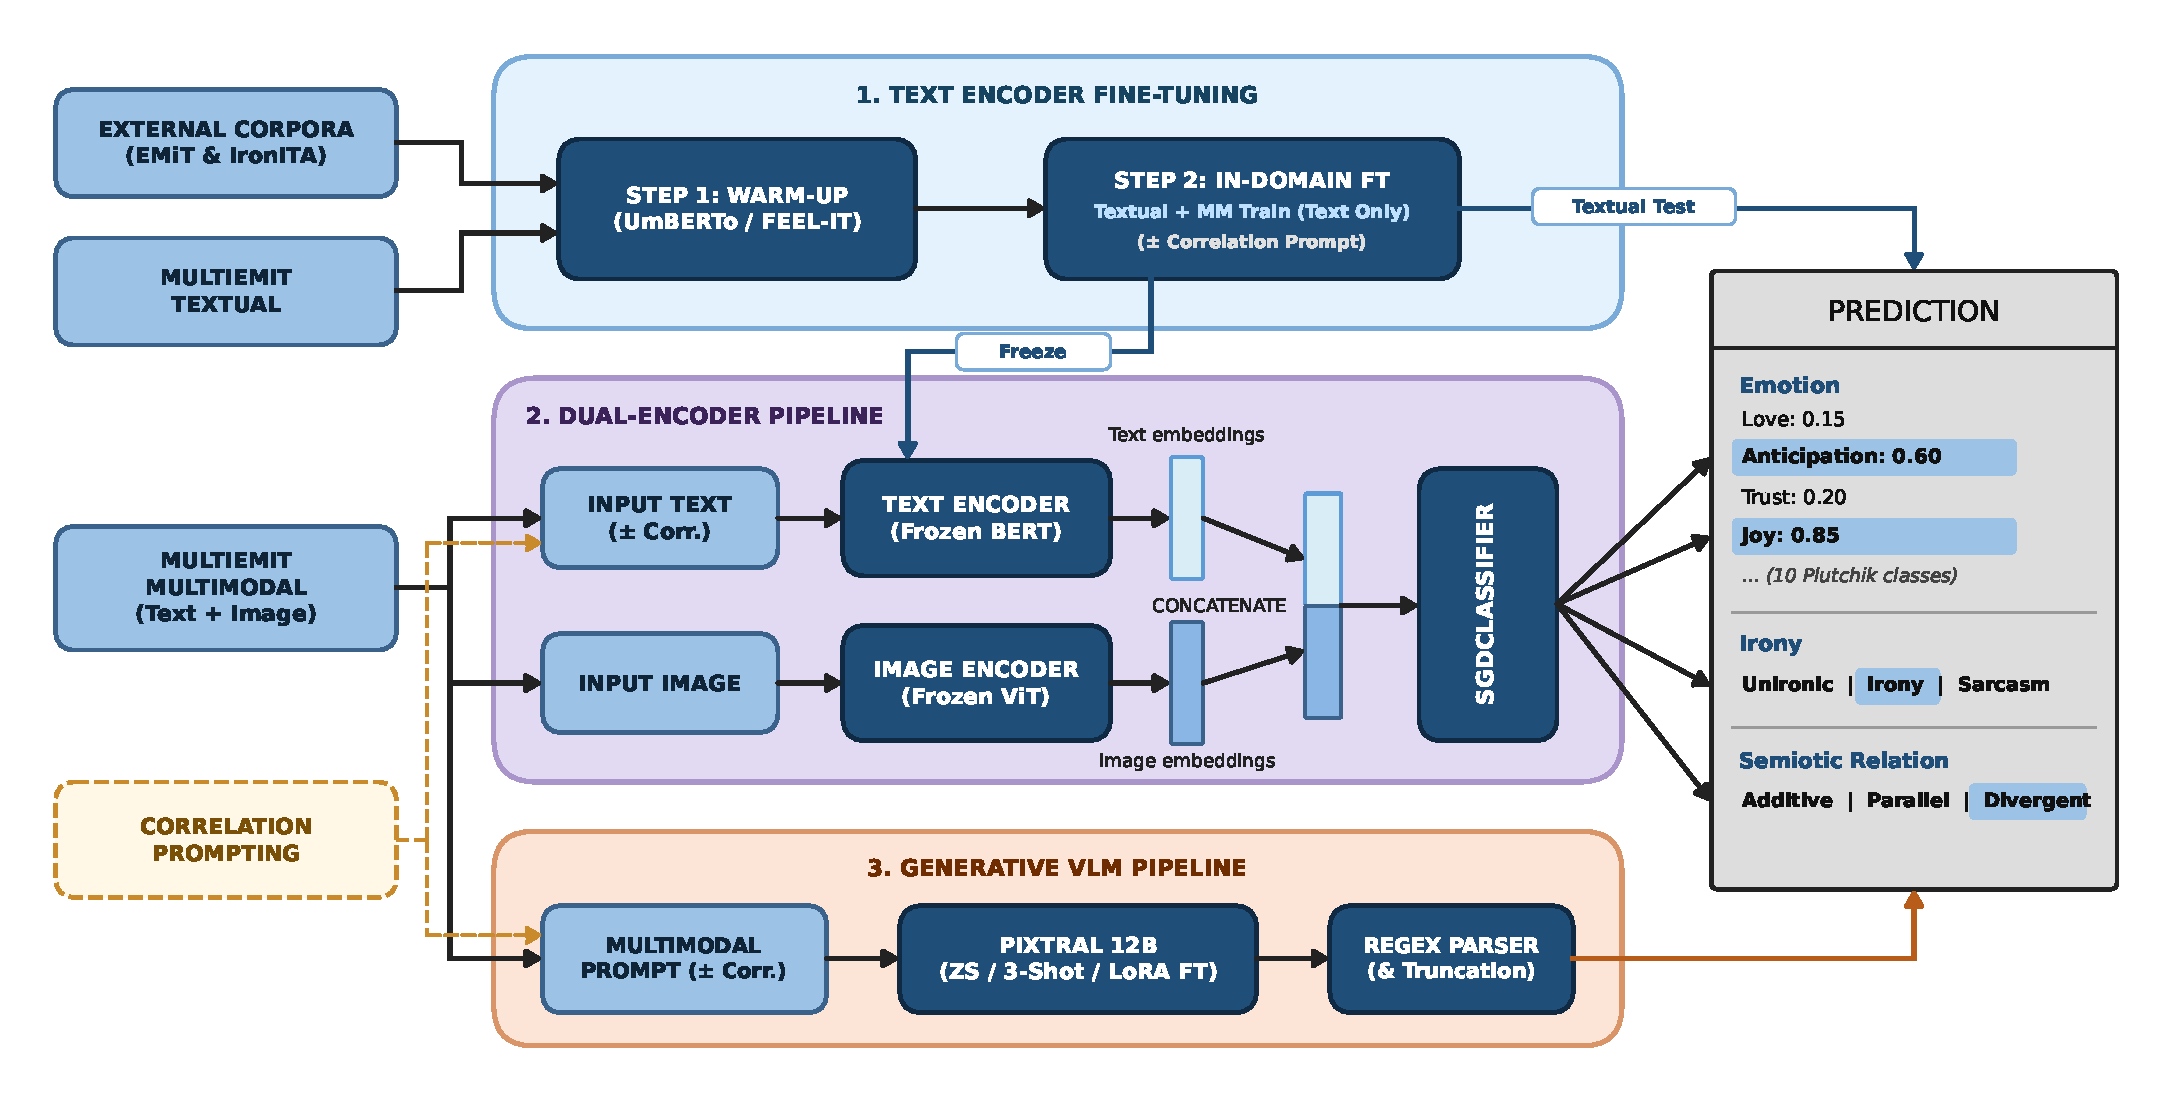
\includegraphics[width=0.92\textwidth]{imgs/pipeline_architecture.pdf}
\caption{Schematic overview of the MultiEMiT experimental pipeline. Text encoders are fine-tuned sequentially in two steps (warm-up on external corpora followed by in-domain fine-tuning on combined MultiEMiT text). For multimodal classification, frozen representations from the fine-tuned text encoder and a frozen ViT image encoder are concatenated into a joint vector ($d=1536$) and classified with linear SVMs (\texttt{SGDClassifier}). The generative pipeline benchmarks Pixtral 12B under zero-shot, few-shot, and LoRA fine-tuning. Correlation prompting optionally verbalizes gold auxiliary annotations across both paradigms.}
\label{fig:pipeline_architecture}
\end{figure*}

This section details the methodology used to probe the MultiEMiT corpus on three tasks: Emotion Detection (multi-label over ten categories), Irony Detection (three mutually exclusive classes: \textit{Unironic}, \textit{Irony}, \textit{Sarcasm}), and Semiotic Relation Detection (\textit{Additive}, \textit{Parallel}, \textit{Divergent}). Rather than maximizing performance, the experiments are designed to measure how much information each modality and each annotation layer carries. All MultiEMiT partitions were split with a fixed 80/20 ratio (\texttt{random\_state=42}): the textual dataset into 1,618 training and 405 test posts, and the multimodal dataset into 516 training and 129 test posts. The same multimodal test split is used for all discriminative and generative models. Given the size of the corpus, no separate validation split was held out. External corpora were used for training only, and all results are computed exclusively on MultiEMiT test instances. An overview of the complete experimental workflow across text-only fine-tuning, discriminative dual-encoding, and generative vision--language modeling is illustrated in Fig.~\ref{fig:pipeline_architecture}.

Because of severe class imbalance, raw accuracy is a misleading indicator of model quality. \textbf{Macro $F_1$} is our primary metric, as it weights all classes equally and penalizes poor performance on minority labels; \textbf{Micro $F_1$} is reported alongside it in the discriminative baseline tables. For reference against class skew, a trivial majority-class baseline on the multimodal test set predicting \textit{Unironic} for all instances achieves an artificially inflated Micro $F_1$ of $0.806$ but a Macro $F_1$ of only $0.298$; on relation detection, predicting the dominant \textit{Additive} class yields Micro $F_1 = 0.527$ and Macro $F_1 = 0.230$. For breakdowns across semiotic subsets (Section~\ref{sec:results}), we report Micro $F_1$ to maintain statistical stability on small subsets; for the single-label irony task, subset Micro $F_1$ equals accuracy, while for relation detection, where subsets coincide with target classes, we report per-class $F_1$. Discriminative results are averaged over three training seeds (42, 123, 456), which control encoder fine-tuning, data ordering, and the linear classifier, while the data splits are kept fixed; this isolates training variability from test-set sampling.

For Emotion and Irony Detection, text encoders were trained in two sequential steps (Fig.~\ref{fig:pipeline_architecture}, top). In \textit{Step~1} (domain warm-up), the encoder was fine-tuned on the union of the MultiEMiT textual training split (1,618 posts) and the full external corpus: EVALITA 2023 EMiT \cite{emit} (5,966 posts) for emotion, and IronITA \cite{ironita2018} (4,849 posts) for irony. In \textit{Step~2}, the Step~1 checkpoint was further fine-tuned on the textual and multimodal training splits (2,134 posts, text only), either on raw text or with correlation-prompted inputs (described below). For Semiotic Relation Detection, where annotations exist only for posts with paired media, UmBERTo encoders were fine-tuned on the multimodal training split, with and without correlation prompts.

Emotion encoders start from the FEEL-IT emotion classifier \cite{bianchi2021feel} (\texttt{MilaNLProc/feel-it-italian-emotion}, based on UmBERTo), while irony and relation encoders start from UmBERTo \cite{musixmatch-2020-umberto}, a RoBERTa-based model \cite{liu2019roberta} pre-trained on Italian Common Crawl with whole-word masking. All encoders were fine-tuned for 10 epochs (batch size 16, learning rate $2\times10^{-5}$, weight decay 0.01, maximum length 128 tokens). For textual emotion inference, labels with sigmoid probability $\geq 0.40$ are predicted; if none exceeds the threshold, the top-ranked label is selected, together with the second one when their probability gap is $\leq 0.10$. The classification heads of these fine-tuned encoders provide the text-only results on the textual test set.

To capture cross-modal interactions, we implemented a discriminative Dual-Encoder pipeline (Fig.~\ref{fig:pipeline_architecture}, middle) operating on frozen features. The last-layer \texttt{[CLS]} embedding of the fine-tuned text encoder (768-d) \cite{devlin2019bert} and the last-layer \texttt{[CLS]} embedding of ViT-Base-224 (\texttt{google/vit-base-patch16-224}) \cite{dosovitskiy2021vit} (768-d; images standardized to $224\times224$ pixels via bilinear resizing without aspect-ratio padding and ImageNet-normalized \cite{deng2009imagenet}) are concatenated, without rescaling, into a 1,536-dimensional vector. A linear SVM (\texttt{SGDClassifier} \cite{pedregosa2011scikit}, squared hinge loss, L2 penalty, balanced class weights) is fitted on the multimodal training split, wrapped in a \texttt{ClassifierChain} \cite{read2011classifier} for multi-label emotion detection to model label interdependencies, and applied directly to the single-label irony and relation tasks. The \textit{text only} configurations apply the same classifier to the text embedding alone, isolating the contribution of the visual features.

Motivated by the cross-layer dependencies observed in Section~\ref{sec:dataset_analysis}, we developed a \textit{Correlation Prompting} strategy tailored to each model family. For discriminative encoders, the gold annotations of the non-target layers are verbalized and prepended to the post (e.g., \textit{``ma soleil è con sua nonna?''} is preceded by \textit{``il seguente testo contiene ironia [...]''}), so that supervised training can learn their statistical association with the target labels. For Emotion and Irony Detection, the verbalization covers the emotion, irony, offensiveness, and target layers (excluding the task being predicted) but not the semiotic relation, which is annotated only for posts with paired media. This keeps the input format identical across the textual and multimodal partitions and prevents image-derived information from entering the text-only configurations; the effect of additionally verbalizing the relation for multimodal posts is reported as an ablation. For Semiotic Relation Detection, all four remaining layers are verbalized. Because gold auxiliary labels are supplied at both training and inference time, correlation prompting is an \textit{oracle} setting that estimates the informativeness of each annotation layer rather than a deployable system.

To compare specialized discriminative systems with modern generative vision--language models, we benchmarked \textbf{Pixtral 12B} \cite{pixtral} (Fig.~\ref{fig:pipeline_architecture}, bottom), an open-weights multimodal language model based on Mistral Nemo with a dedicated 400M-parameter vision encoder. Pixtral was fine-tuned and evaluated exclusively on the multimodal partition, using the same test split as the Dual-Encoder. Since its training data and input format differ from those of the discriminative pipeline, this comparison contrasts modeling paradigms on a shared test set rather than constituting a controlled ablation. In correlation-prompted settings, each post is preceded by the verbalized annotations of the other layers, always including the semiotic relation for emotion and irony, at both training and inference time. A fine-tuned encoder can learn statistical associations between these annotations and the target labels, but a model used in zero- or few-shot inference cannot. We therefore emulate this learned knowledge by additionally stating in the task instruction the main Pearson correlations between the target labels and the other annotation layers (e.g., \textit{``Disgust correlates with Sarcasm. Anger correlates with Offensivity.''}; see Section~\ref{sec:dataset_analysis}). To measure prompt sensitivity, we designed five variants spanning three correlation intensity thresholds: \textbf{Short} ($|r| \ge 0.25$), \textbf{Medium} ($|r| \ge 0.20$), and three \textbf{Long} formulations (\textit{long\_v1}, \textit{long\_v2}, \textit{long\_v3}; $|r| \ge 0.15$). Following findings from the BRIGHTER benchmark \cite{brighter_project} showing that multilingual LLMs exhibit stronger instruction adherence when prompted in English, all generative instructions were formulated in English.

For all Pixtral experiments, input images were standardized to a fixed resolution of $336 \times 336$ pixels via the model's image processor (\texttt{size = \{"height": 336, "width": 336\}}). We evaluated Pixtral across three regimes: Zero-Shot Prompting across all five correlation variants and an unprompted baseline; Few-Shot (Three-Shot) Prompting \cite{brown2020language} for Semiotic Relation Detection, where three complete multimodal examples were included in the prompt as a design choice to help the model with a newer and more specialized task that it is less likely to have encountered during pre-training compared to emotions or irony; and LoRA Fine-Tuning on the MultiEMiT multimodal training set ($r=16$, $\alpha=32$, RSLoRA \cite{hu2021lora, kalajdzievski2023rank}, all linear target modules, dropout $0.1$), adapting 66,322,432 parameters out of 12.75 billion (0.52\% trainable) with per-device batch size 1, 8 gradient accumulation steps, learning rate $3 \times 10^{-5}$, FP16 mixed precision, and gradient checkpointing over 2 epochs. To account for generation variance, each Pixtral configuration was evaluated at two decoding temperatures ($T=0.1$ and $T=0.9$) with 3 independent runs per setting (reporting mean scores). To extract predictions from the generated text, we used regular expressions to match valid label names. After fine-tuning on emotion detection, Pixtral often continued generating long or repeated lists of emotions instead of stopping after one or two labels. Because regex matching extracted all mentioned labels, these extra guesses lowered performance. By comparing the raw outputs with the gold labels, we noticed that the emotions were usually listed from most likely to least likely, so we added a truncation parameter that keeps only the first $n=2$ distinct emotions, matching the maximum of two emotions requested in the prompt.